\graphicspath{{sections/MARVINWOLF/images/}}

\section[Ausführen des Programms]{Ausführen des Programms\myAuthor{Marvin Wolf}}
Wie die Entwicklungsumgebung aufgesetzt und das Programm gestartet wird, ist in der Datei README.md im Wurzelverzeichnis des Projekts beschrieben.\\ \\
Nach dem Start zeigt die Master-Node GUI den Zustand aller ROS Nodes. Sobald alle bereit sind, wird der Ablauf über ”Run” gestartet.
\begin{figure}[ht]
    \centering
    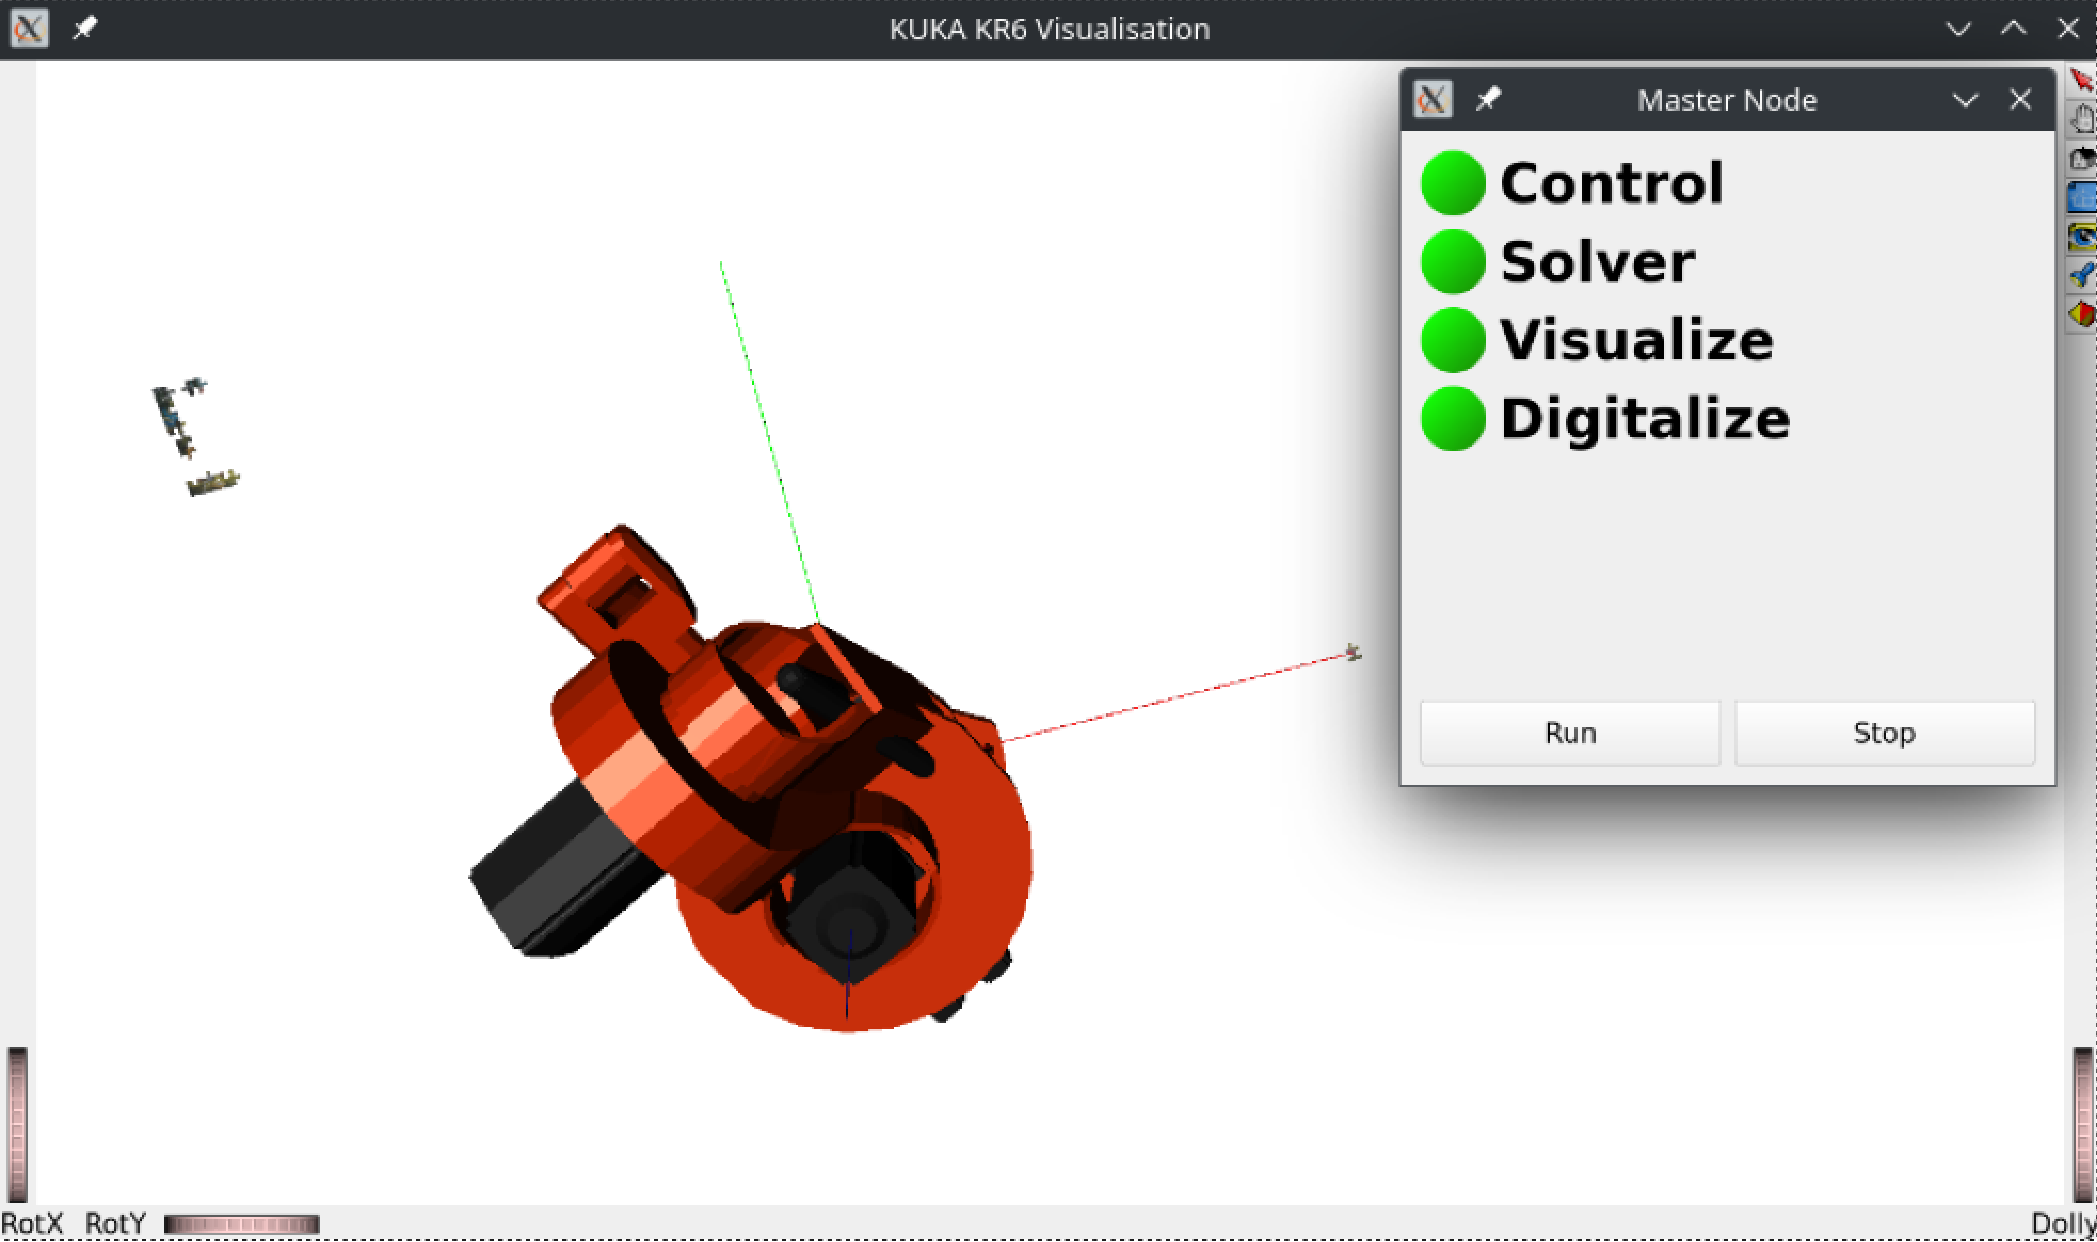
\includegraphics[width=1\textwidth]{masternoderunning.png}
    \caption{Master-Node sowie Roboter}
\end{figure}\\
Nach Ablauf des Programms ist das Puzzle gelöst und korrekt angeordnet auf dem Boden ausgebreitet.
\begin{figure}[H]
  \centering
  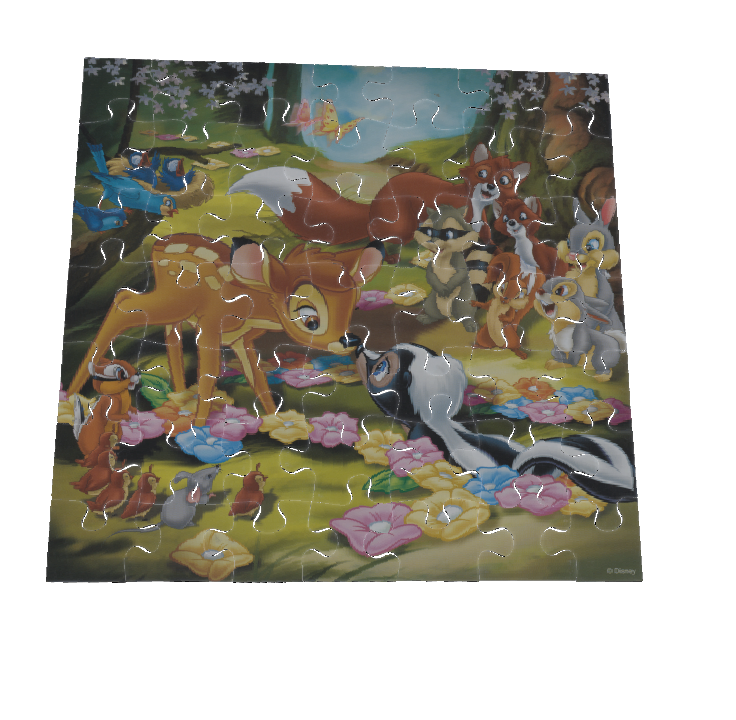
\includegraphics[width=1\textwidth]{solvedpuzzle.png}
  \caption{Endergebnis}
\end{figure}
